
\section{Les frottements solides}
\label{sec:frot}

\subsection{Que sont les frottements ?}

Les termes de \textit{frottement} ou de \textit{friction} désignent l'ensemble des interactions qui s'appliquent à deux systèmes mécaniques en contact et qui s'opposent à leur mouvement.
Le domaine de la physique qui étudie les frottements solides, la \textit{tribologie}, est définie comme la science de l'usure, des frottements et de la lubrification.
%Les phénomènes de frottement sont omniprésents tant dans notre quotidien que dans les applications technologiques de pointe ou les évènements géophysiques
Ces phénomènes sont omniprésents dans notre quotidien. Nous les retrouvons par exemple dans le simple fait de marcher, puisque c'est l'existence d'un frottement solide entre nos chaussures et le sol qui nous propulse en avant. Ceci est bien illustré par la grande difficulté avec laquelle
%\href{https://youtu.be/qQE-lMtGaN8}{\textcolor{black}{nous nous déplaçons sur la glace}},
nous nous déplaçons sur la glace,
surface à frottements faibles\,\cite{bowden_friction_1953}.


Cette section discute, par une approche historique, des mécanismes et modélisations du frottement solide. Ces mécanismes sont une première approche de la mécanique des failles, en particulier des séismes, qui peuvent être décrits comme la manifestation d'un mouvement de stick-slip, caractéristique des interfaces frictionnelles\,\cite{brace_stick-slip_1966}. 

\subsection{Origine microscopique des forces de frottement macroscopiques}

\begin{figure}[htb]
\centering
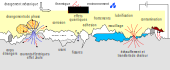
\includegraphics[scale=1]{../Figures_chap_intro/microscopic_complexity.pdf}
\caption[Complexité d'une interface réelle]{Visualisation schématique d'un contact frictionnel réel, et des interactions à l'œuvre à l'interface. L'aire de contact réelle entre les deux solides est nettement plus faible que l'aire de contact apparente.}
\label{fig:asperit}
\end{figure}




Lors d'un contact frictionnel entre deux objets, les frottements solides se manifestent à l'échelle macroscopique par l'apparition d'une force opposée à leur mouvement relatif. L'origine de cette force est à chercher à l'échelle microscopique. Une surface qui nous apparaît lisse au toucher est en réalité rugueuse, couverte d'aspérités dont la position et la taille sont aléatoires, à la manière d'un papier abrasif microscopique, allant selon les matériaux et traitements de surfaces du nanomètre au millimètre. Lors de la mise en contact de deux solides, ces aspérités s'entremêlent, répartissant la force pressante sur de multiples points de contacts, nommés \textit{microcontacts}. Ces points sont le siège d'un ensemble complexe d'interactions électrostatiques, chimiques et mécaniques, dans lesquelles interviennent les deux surfaces rugueuses des solides, mais également les impuretés et corps étrangers présents entres ceux-ci (Fig.\,\ref{fig:asperit}). La complexité de ces interactions rend irréaliste l'étude du comportement d'une interface rugueuse par le calcul exact de toutes les forces qui s'y exercent. L'étude de ces interfaces s'est donc historiquement faite au travers de lois empiriques macroscopiques telles que les lois d'Amontons-Coulomb (Sec.\,\ref{sec:coulomb}), puis par des lois justifiées par des modèles microscopiques des contacts à l'interface, comme le modèle de Bowden et Tabor, puis les modèles dits \textit{Rate-and-State} (Sec.\,\ref{sec:microfric}).

La prochaine section est dédiée aux premières tentatives de la modélisation de la friction solide par les lois d'Amontons-Coulomb.


\subsection{Description macroscopique -- Lois d'Amontons-Coulomb}
\label{sec:coulomb}


\begin{figure}[htb]
\centering
\includegraphics[width=.45\textwidth]{../Figures_chap_intro/vinci.png}
\caption[Croquis de Léonard de Vinci]{Croquis de Léonard de Vinci au sujet du frottement d'un objet sur une surface. Les dessins représentent des expériences d'étude de la friction par traction dans lesquelles différents objets sont tractés par une masse leur étant reliée par une cordelette et une poulie (adapté de\,\cite{hutchings_leonardo_2016}).}
\label{fig:vinci}
\end{figure}

Bien que les premiers écrits sur les frottements solides remontent à l'antiquité romaine, Thémistios écrivant notamment au quatrième siècle dans son \textit{De la Physique} «\,Il est plus facile d'entretenir le mouvement d'un corps se déplaçant que d'initier celui d'un corps au repos\,»\,\cite{themistius_aristotle_2008}, la première modélisation des frottements solides est due à Léonard de Vinci au XV\up{ème} siècle, dans son \textit{Codex Atlanticus} (Fig.\,\ref{fig:vinci})\,\cite{hutchings_leonardo_2016}. Ces travaux, redécouverts par Guillaume Amontons en 1699, et complétés par Leonhard Euler (1750) et Charles-Augustin de Coulomb (1785), ont abouti à la modélisation du problème à deux corps en contact frictionnel et à l'établissement de trois lois macroscopiques permettant de le résoudre.

\subsubsection{Définition du problème}

\begin{figure}[htb]
\centering
\includegraphics[scale=1]{../Figures_chap_intro/coulomb.pdf}
\caption[Référentiel utilisé pour les lois de Coulomb]{Définition du système étudié. Le référentiel choisi est celui du laboratoire muni d'un repère orthonormé direct $\left(\vec{e_x},\,\vec{e_y},\,\vec{e_z}\right)$. Le plan dans lequel le contact entre la masse et la surface s'effectue est le plan  $\left(\vec{e_x},\,\vec{e_z}\right)$, et $\vec{e_y}$ est pris orthogonal à ce plan, et orienté vers le haut (et de manière plus générale dans la direction opposée à la force pressante).
}
\label{fig:coulomb}
\end{figure}

Le système que nous considérons dans le cadre de la friction entre deux solides est une masse $m$ indéformable dont la surface macroscopiquement lisse d'aire $A$ est déposée sur un support horizontal immobile (Fig.\,\ref{fig:coulomb}). Sa vitesse est notée $\vec{v}$, et la direction de la vitesse $\vec{u_v} = \vec{v}/\norm{\vec{v}}$. Nous nommons \textit{force normale} $\vec{F_N}$, ou force pressante, la projection de la somme des forces appliquées à la masse sur le vecteur normal à l'interface, en excluant la réaction du support.

Les phénomènes de friction entrent en jeu lorsqu'une force tend à mettre en mouvement le solide, et a donc une composante tangentielle à l'interface. Ils se manifestent par l'apparition d'une force $\vec{F_f}$, qui s'applique dans le plan de l'interface, dans la direction contraire au sens de la mise en mouvement. Nous nommerons alors \textit{force cisaillante} $\vec{F_S}$ la projection de toutes les forces appliquées à la masse dans le plan de l'interface, à l'exception de cette force de réaction due aux frottements (Fig.\,\ref{fig:coulomb}).

Le problème étant ainsi défini, nous pouvons énoncer les trois lois d'Amontons-Coulomb décrivant la force de frottement $\vec{F_f}$ en fonction des forces normale $\vec{F_N}$ et cisaillante $\vec{F_S}$ appliquées à la masse $m$.


\subsubsection{Lois d'Amontons-Coulomb}

La modélisation du comportement d'une interface frictionnelle repose sur trois lois fondamentales, nommées d'après ceux qui les ont découvertes et rendues publiques, Guillaume Amontons (1699) et Charles-Augustin de Coulomb (1785).

\myparagraph{Lois du frottement statique -- \boldmath$\mu_s$}

La première loi d'Amontons affirme que pour mettre en mouvement la masse lorsqu'elle est immobile, il faut lui appliquer une force cisaillante telle que $F_S=\mu_sF_N$, où $\mu_s$ est une constante nommée \textit{coefficient de frottement statique}. Elle s'écrit

\begin{equation}
\text{tant que }{v}=0\qquad
\begin{aligned}\left\{
	\begin{split}
		\max F_f &= \mu_s F_N\\
		\vec{F_f} &= -\vec{F_S}\\
	\end{split}
	\right.
\end{aligned}
\end{equation}


La deuxième loi d'Amontons stipule que la force de frottement, notamment $\mu_s$, ne dépend pas de l'aire de contact apparente entre les deux solides.


\myparagraph{Loi du frottement dynamique -- \boldmath$\mu_d$}


La troisième loi de la friction, ou loi de Coulomb, précise qu'une fois que le solide est mis en mouvement relativement au support, la force de frottement qu'il subit est toujours opposée à la direction du mouvement et de norme constante, indépendante notamment de sa vitesse de glissement. Cette troisième loi nous permet de définir le \textit{coefficient de frottement dynamique} $\mu_d$ tel que

\begin{equation}
\vec{F_f} = - \mu_d F_N\,\vec{u_v}
\end{equation}


Une conséquence intéressante de cette loi est que la force de frottement est non-conservative, puisque son travail dépend du chemin suivi par l'objet sur lequel elle s'applique. Sur un chemin $\mathscr{C}$ de longueur $L_{\mathscr{C}}$,  à force normale constante, le travail $W_{\mathscr{C}}(\vec{F_f})$ vaut


\begin{equation}
W_{\mathscr{C}}(\vec{F_f})
= \int_{\mathscr{C}}\vec{F_f}\cdot\mathrm{d}\vec{u_v}
= -\mu_dF_N
\times \int_{\mathscr{C}}\vec{u_v}\cdot\mathrm{d}\vec{u_v} 
= -\mu_dF_NL_{\mathscr{C}}
\label{eq:dissip}
\end{equation}

Ce travail étant toujours négatif, la force de frottement dynamique fait toujours perdre au système de l'énergie. L'énergie perdue, dissipée en chaleur, est proportionnelle à la distance parcourue par l'objet.




\subsubsection{Variabilité des coefficients de frottement}

Émergeant des lois d'Amontons-Coulomb, $\mu_s$ et $\mu_d$ peuvent être considérés comme des grandeurs caractéristiques d'une interface entre deux matériaux donnés. Selon les conditions expérimentales (état de surface, lubrification, humidité ambiante, etc.) ces coefficients varient, mais à conditions expérimentales fixées il est possible de tabuler leurs valeurs (Fig.\ref{table:coef}). Cependant même en conditions expérimentales contrôlées, les coefficients varient d'un échantillon à un autre, et d'une expérience à l'autre, d'un facteur typiquement de l'ordre de 10\%, et leur utilisation nécessite un regard critique\,\cite{ben-david_static_2011, blau_significance_2001, czichos_multilaboratory_1987} (Fig.\,\ref{fig:disparite}). L'indépendance de $\mu_d$ de la vitesse de glissement notamment est une approximation dont les limites sont expérimentalement observées (Sec.\,\ref{sec:evolutionmacro}).


% Émergeant des lois d'Amontons-Coulomb, $\mu_s$ et $\mu_d$ sont souvent considérés comme des grandeurs caractéristiques d'une interface entre deux matériaux donnés. En réalité ils dépendent des conditions expérimentales dans lesquelles les deux matériaux sont frottés, en particulier de l'état de surface de ceux-ci, ou de la présence de corps étrangers. Ces variations donnent lieu à des tables de valeurs de coefficients de frottement entre différents matériaux et dans différentes conditions (Fig.\ref{table:coef}). Même en conditions contrôlées, ces coefficients sont très variables d'un échantillon à l'autre, et d'une expérience à l'autre, et leur utilisation nécessite un regard critique\,\cite{ben-david_static_2011, blau_significance_2001, czichos_multilaboratory_1987} (Fig.\,\ref{fig:disparite}). L'indépendance de $\mu_d$ de la vitesse de glissement notamment est une approximation dont les limites sont expérimentalement observées (Sec.\,\ref{sec:evolutionmacro}).

\begin{figure}[htb]
\centering
\begin{tabular}{ |p{4.5cm}||p{3cm}|p{3cm}|  }
 \hline
 \multicolumn{3}{|c|}{Coefficient de frottement statique} \\
 \hline
 \textbf{Matériau de la corde}& \textbf{Sèche} & \textbf{Humide} \\
 \hline
 Nylon         & 0.10 -- 0.12 &  0.12 -- 0.15\\
 Polyester     & 0.12 -- 0.15 &  0.15 -- 0.17\\
 Polypropylène & 0.08 -- 0.11 &  0.08 -- 0.11\\
 Aramide        & 0.12 -- 0.15 &  0.15 -- 0.17\\
 HMPE          & 0.08 -- 0.11 &  0.08 -- 0.11\\
 \hline
\end{tabular}
\caption[Exemple de table de coefficients de frottement statique]{Exemple de table de coefficients de frottement statique. Sont tabulés ici les coefficients de frottement entre une plaque d'acier lisse et des cordes de différents matériaux, sèches ou humides\,\cite{mckenna_properties_2004}.}
\label{table:coef}
\end{figure}

\begin{figure}[htb]
\centering
\includegraphics[width=.6\textwidth]{../Figures_chap_intro/multilab.png}
\caption[Variabilité du coefficient de frottement]{Coefficients de frottement dynamique mesurés par différentes équipes de recherche sur des échantillons identiques en acier. Chaque point représente une expérience, et chaque colonne de points l'ensemble des résultats d'un laboratoire (extrait de\,\cite{ czichos_multilaboratory_1987}). Moyenne : $0.6$, écart type : $0.109$.}
\label{fig:disparite}
\end{figure}




\subsubsection{Émergence du phénomène de stick-slip}
\label{sec:ss1}

\begin{figure}[htb]
\centering
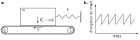
\includegraphics[scale=1]{../Figures_chap_intro/stickslip.pdf}
\caption[Mouvement de stick-slip sur un tapis roulant]{\textbf{a.} Système mécanique pouvant aboutir à un mouvement de stick-slip. \textbf{b.} Évolution temporelle typique de la longueur du ressort dans ce système. Les axes sont en unités arbitraires, de tels mouvements pouvant se produire à des échelles très variées.}
\label{fig:shemastickslip}
\end{figure}

Le phénomène de stick-slip, ou collé-glissé, est un mouvement saccadé entre deux solides liés par une interface frictionnelle, qui émerge de la différence entre $\mu_s$ et $\mu_d$.
Pour le mettre en évidence, considérons un système modèle composé d'une masse $m$, reliée à un support immobile par un ressort idéal de raideur $k$, et placée sur un tapis roulant évoluant à vitesse constante $v$ (Fig.\,\ref{fig:shemastickslip}). Alors si $\mu_d<\mu_s$, le mouvement se décompose en deux phases qui alternent :

\begin{itemize}
\bitem \textit{Stick} : les deux solides sont solidaires, leur mouvement relatif est nul, les lois d'Amontons décrivent les interactions frictionnelles entre les deux par le biais du coefficient de frottement statique $\mu_s$. Durant cette phase, l'interface se charge en cisaillement par les déformations du ressort.
\bitem \textit{Slip} : les deux solides se mettent en mouvement relatif, ils glissent, la troisième loi de Coulomb décrit le mouvement par le coefficient $\mu_d$.
\end{itemize}


Les lois d'Amontons Coulomb permettent d'aboutir à la description d'un mouvement périodique, de période $T_{ss}$,  et d'amplitude $A_{ss}$, qui en posant $\omega_0 = \sqrt{{k}/{m}}$ s'écrivent


\begin{align}[left=\empheqlbrace]
	\begin{split}
		T_{ss} &= 2\frac{(\mu_s-\mu_d) \,g}{\omega_0^2\,v} + \dfrac{\pi}{\omega_0}\\
		A_{ss} &= \frac{(\mu_s-\mu_d)\,g}{\omega_0 ^2}
	\end{split}
\label{eq:freqss}
\end{align}



Les lois d'Amontons-Coulomb permettent de décrire synthétiquement de nombreux systèmes frictionnels, mais sont limitées en raison des variations des coefficients de frottement en fonction du temps et de la vitesse, et de l'hétérogénéité des interfaces réelles. Elles ont été énoncées à leur origine sans justification microscopique, et relèvent d'une description empirique d'interfaces macroscopiques. Un modèle microscopique historiquement utilisé pour les décrire est détaillé dans la section suivante.



\subsection{Modèles microscopiques de la friction}

\label{sec:microfric}



La description par des modèles macroscopiques du frottement entre deux solides s'appuie historiquement sur des observations empiriques. Les modèles microscopiques justifiant de la validité des trois lois d'Amontons-Coulomb sont récents (\textsc{xx}\up{ème} siècle), avec notamment le modèle de Bowden et Tabor\,\cite{bowden_friction_1950}, publié en 1950. Ces modèles reposent sur la prise en compte de la réalité microscopique des contacts entre les deux solides.


\subsubsection{Description de l'aire de contact réelle}

\begin{figure}[h]
\centering	
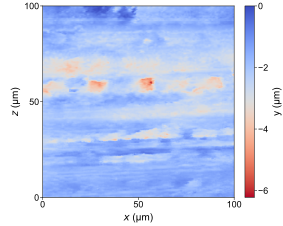
\includegraphics[scale=1]{../Figures_chap_intro/profiloplot_zoom.pdf}
\caption[Profil microscopique d'un bloc de PMMA]{Profil d'altitude d'une portion de bloc de plastique poli  à l'aide de papier abrasif fin (P1200). L'altitude de référence est la surface macroscopique du bloc. Les aspérités, dont la hauteur est de l'ordre de quelques micromètres, semblent aléatoirement distribuées. Cet échantillon présente des traces d'usure, sous la forme de rainures le long de l'axe $x$.}
\label{fig:asperit2}
\end{figure}


Lorsque deux solides sont en contact, l'aire de contact réelle entre les microaspérités à l'interface est bien plus faible que l'aire apparente macroscopique de contact $A$ (Fig.\,\ref{fig:asperit2}). Lors de la mise en contact de deux solides, seules les plus hautes aspérités de chaque surface se rencontrent. L'aire réelle de contact est nommée $A_r$ et peut être décrite comme la somme des aires de chaque aspérité en contact. Cette aire est par exemple mesurable dans les solides transparents par des méthodes optiques reposant sur la réflexion interne totale de la lumière\,\cite{dieterich_direct_1994}.
Afin de modéliser le contact entre les deux solides, un modèle du comportement des microcontacts soumis à une pression et de leur distribution est nécessaire.

La mécanique des contacts est un domaine de recherche riche et actif, et nous n'en proposons dans ce chapitre qu'un aperçu, au travers de deux modèles historiques de contacts uniques. Il  existe cependant d'autres méthodes pour aborder ce type de problèmes, plus récentes et plus précises\,\cite{greenwood_contact_1966, derjaguin_effect_1975,  johnson_surface_1971, maugis_adhesion_1992, persson_theory_2001, vakis_modeling_2018}, que nous n'aborderons pas ici.




Dans cette section, de façon à distinguer les forces macroscopiques $F_N$ et $F_S$ des forces à l'échelle des microcontacts, nous nommerons en minuscule $f_n$ et $f_s$ les forces appliquées sur un microcontact de surface $A_\mu$, de telle sorte qu'une contrainte $\sigma$ subie par ce microcontact s'écrive $\sigma=f/A_\mu$.


\subsubsection{Modèles d'aspérités}




Nous présentons deux modèles d'aspérités sans adhésion, selon que la pression de contact est faible, et les déformations élastiques, ou que la pression est forte, et les déformations plastiques.

\myparagraph{Aspérité élastique}

Pour une aspérité individuelle élastique, de module d'Young $E$ et de coefficient de Poisson $\nu$, nous noterons $E^*={E}/(1-\nu^2)$. Dans le cadre du contact de Hertz\,\cite{hertz_ueber_1882}, si cette aspérité dispose d'un rayon de courbure $\rho_r$ et est pressée contre une surface dure sous une force normale $f_n$, alors son aire de contact avec cette surface est

\begin{equation}
A_\mu = \pi\left(\frac{3}{4}\times\frac{1}{E^*}\times\rho_r\times f_n\right)^{2/3}\propto f_n^{2/3}
\end{equation}



Ainsi l'aire de contact augmente proportionnellement à $f_n^{2/3}$, tandis que la pression subie par le contact, $f_n/A_\mu$, augmente proportionnellement à $f_n^{1/3}$.


\myparagraph{Aspérité plastique}

\begin{figure}[htb]
\centering
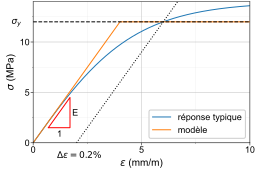
\includegraphics[scale=1]{../Figures_chap_intro/yield.pdf}
\caption[Limite de plasticité d'un matériau]{Réponse contrainte-déformation d'un matériau plastique typique, avec $E=\SI{3}{\giga\pascal}$ et $\sigma_Y=\SI{12}{\mega\pascal}$. En bleu, exemple de réponse typique du matériau. Dans les régimes que nous considérons, la contrainte est une fonction croissante de la déformation. Nous la modélisons par la courbe orange. Ce modèle comporte d'abord une réponse purement élastique, telle que si $\varepsilon<\sigma_Y/E$ alors $\sigma=E\varepsilon$, puis une réponse purement plastique, telle que si $\varepsilon\geq\sigma_Y/E$, alors $\sigma = \sigma_Y$. La définition communément acceptée de $\sigma_Y$, représentée par les lignes pointillées, est la valeur de contrainte telle qu'une fois le matériau de nouveau déchargé, sa déformation plastique soit de 0.2\%\,\cite{avallone_marks_2006}.}
\label{fig:yield}
\end{figure}




Si les contraintes subies par les microcontacts sont grandes les déformations sont plastiques, et $\sigma$ atteint un maximum. La contrainte limite d'élasticité $\sigma_Y$ (\textit{yield stress}, homogène à une pression) est définie comme la contrainte à partir de laquelle les déformations de l'aspérité deviennent plastiques (Fig.\,\ref{fig:yield}). La valeur de $\sigma_Y$ est une caractéristique du matériau. Les valeurs typiques de $\sigma_Y$ sont de l'ordre de quelques $10^7\,\text{Pa}$ pour la plupart des matériaux polymères rigides\,\cite{avallone_marks_2006}. Cela correspond environ à dix fois la contrainte normale que nous appliquons sur la surface \textit{apparente} de nos échantillons expérimentaux (Sec.\,\ref{sec:echantillons}).

Si une force normale $f_n$ est appliquée sur un microcontact plastique de surface de contact $A_{\mu}$, celle-ci ne pouvant supporter qu'une contrainte normale $\sigma_n=\sigma_Y$, alors

\begin{equation}
A_\mu = \frac{f_n}{\sigma_Y}
\label{eq:microcontact}
\end{equation}

Ainsi, $A_\mu$ augmente linéairement avec $f_n$.


\myparagraph{Cisaillement d'une aspérité}

Qu'il soit élastique ou plastique, un microcontact résiste au glissement tant qu'il n'est pas brisé ou affaibli. Sa résistance au cisaillement $\sigma_r$ correspond à la contrainte cisaillante maximale qu'il peut supporter sans glisser. La force cisaillante $f_s$ maximum que le microcontact peut retenir est donc

\begin{equation}
\max f_s = A_\mu\times \sigma_r
\end{equation}

Ainsi la force cisaillante maximale que peut supporter un microcontact avant de glisser augmente linéairement avec $A_\mu$.

\pagebreak

En conclusion, ces deux modèles montrent que la surface d'un microcontact augmente avec la force normale qu'il porte. Elle est proportionnelle à la force normale dans le cas d'un microcontact plastique, tandis que pour un microcontact élastique elle est proportionnelle à $f_n^{2/3}$. La force cisaillante que peut retenir un microcontact est pour sa part proportionnelle à cette surface. Ces modèles de microcontacts peuvent maintenant être appliqués à l'échelle d'une interface toute entière.




\subsubsection[Modèle d'interface -- lois d'Amontons-Coulomb]{Modèle d'interface -- justification des lois d'Amontons-Coulomb}
\label{sec:amontonsmicro}

Nous restreignons cette présentation au cas d'une interface dont les contacts ont un comportement plastique car les matériaux que nous étudions dans les conditions choisies sont correctement décrits par ce modèle\,\cite{rubinstein_crack-like_2006}. Cependant les résultats présentés resteraient valides pour une interface partiellement ou entièrement élastique avec une distribution gaussienne des hauteurs des aspérités\,\cite{singer_contact_1992}.

\myparagraph{Frottement statique}

Dans le cas d'une interface plastique, le modèle de Bowden et Tabor\,\cite{bowden_friction_1950} décrit la surface comme un ensemble de microcontacts de surfaces $\{A_{\mu,i}\}_i$. La force normale portée par l'interface peut alors s'écrire comme la somme des forces normales portées par l'ensemble des microcontacts, $F_N = \sum_if_{n,i}$. En appliquant l'Équation\:\ref{eq:microcontact} à chacun de ces microcontacts nous obtenons

\begin{equation}
A_r = \sum_i A_{\mu,i} = \sum_i\frac{f_{n,i}}{\sigma_Y} = \frac{F_N}{\sigma_Y}
\label{eq:wamu}
\end{equation}

Ainsi l'aire de contact réelle $A_r$ de l'interface est proportionnelle à la force normale $F_N$ qui lui est appliquée. En appliquant un raisonnement similaire sur la force cisaillante, répartie sur tous les microcontacts, nous obtenons $\max F_S = \sum_i \max f_{s,i} = \sum_i  \sigma_rA_{\mu,i} = \sigma_r A_r$. Ainsi le coefficient de frottement statique se définit comme

\begin{equation}
\max F_S = \mu_sF_N\qquad\text{avec} \qquad \mu_s = \dfrac{\sigma_r}{\sigma_Y}
\label{eq:maxfs1}
\end{equation}



Au travers cette modélisation microscopique nous retrouvons les deux lois d'Amontons, ainsi qu'une définition du coefficient de frottement statique. Cette définition reste sujette à discussion, puisqu'elle repose sur l'utilisation de $\sigma_Y$ et $\sigma_r$. La contrainte limite d'élasticité $\sigma_Y$ est une caractéristique du matériau, et la considérer constante est une bonne approximation. La résistance au cisaillement $\sigma_r$ pour sa part n'est pas une grandeur caractéristique. Elle dépend de la géométrie des contacts et de chaque aspérité considérée, et n'est pas à priori connue.


\myparagraph{Frottement dynamique}


Lorsque l'interface est en glissement quasi-statique, les microcontacts se cassent et se reforment de manière répétée. La formation d'un point de contact s'accompagne de l'accumulation rapide de contraintes cisaillantes sur ce point, puis à une nouvelle mise en glissement. Les deux aspérités poursuivent leur glissement jusqu'à rencontrer une nouvelle aspérité avec laquelle répéter ce cycle. Tandis que le solide glisse de manière quasi-statique, les microcontacts subissent des mouvements rapides et irréguliers\,\cite{persson_sliding_1998,beig_friction_2006}. En reprenant la description du contact unique cisaillé proposée plus haut (Éq.\,\ref{eq:wamu} et\,\ref{eq:maxfs1}), chaque rupture de microcontact s'effectue à une force cisaillante $f_s$ telle que

\begin{equation}
f_s=A_\mu\times\sigma_r= \dfrac{\sigma_r}{\sigma_Y}f_n
\end{equation}

Ainsi, peu importe la vitesse à laquelle le glissement est effectué, si nous considérons comme isotrope la répartition des microcontacts, la force cisaillante macroscopique $F_S$ est de valeur constante

\begin{equation}
F_S = \mu_dF_N\qquad\text{avec} \qquad \mu_d = \mu_s = \dfrac{\sigma_r}{\sigma_Y}
\label{eq:maxfs}
\end{equation}


Les limitations de ce modèle sont ainsi mises en exergue, puisqu'il ne parvient pas à prédire de différence entre $\mu_s$ et $\mu_d$, ni l'évolution de ces deux coefficients en fonction du temps et de la vitesse de glissement observée expérimentalement pour des interfaces solide-solide réelles.



\subsection[Modélisation de l'évolution de $\mu$]{Modélisation de l'évolution des coefficients de frottement}
\label{sec:evolutionmacro}

Les coefficients de frottement ne sont pas des caractéristiques d'une interface, comme décrit précédemment. Le coefficient de frottement statique tend à augmenter avec l'âge de l'interface, tandis que le coefficient de frottement dynamique, à l'inverse de ce que stipule la troisième loi de Coulomb, dépend de la vitesse de glissement. Cette section décrit ces observations et un modèle empirique permettant d'en rendre compte.

\subsubsection{Vieillissement d'une interface au repos}
\label{sec:aging}

\begin{figure}[htb]
\centering
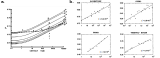
\includegraphics[scale=1]{../Figures_chap_intro/aging.pdf}
\caption[Vieillissement d'une interface bloquée]{\textbf{a.} Évolution du coefficient de frottement statique $\mu$ en fonction du temps de contact normalisé ($\tau=\theta/\theta_0$) pour différentes roches (extrait de\,\cite{dieterich_modeling_1979}). Les échantillons étudiés sont des granodiorites californiennes poncées avec des papiers abrasifs P60 à P600. Pour tous les échantillons présentés, le coefficient augmente proportionnellement au logarithme de l'âge de l'interface. \textbf{b.} Évolution du coefficient de frottement statique $\mu_s$ en fonction du temps de contact $\tau$ dans divers matériaux (extrait de\,\cite{baumberger_contact_1997}). La ligne est un ajustement des points de la forme $\mu(\tau)=\mu_0+\text{b}\ln\tau$.}
\label{fig:aging}
\end{figure}



Le coefficient de frottement statique augmente logarithmiquement avec le temps de contact entre les deux solides (Fig.\,\ref{fig:aging}), dans tous les matériaux, y compris les roches et les matières plastiques\,\cite{dieterich_modeling_1979,baumberger_contact_1997} comme le polyméthacrylate de méthyle (PMMA) que nous utilisons dans nos expériences (Sec.\,\ref{sec:materials}). Ce vieillissement (\textit{aging}) s'explique par une augmentation logarithmique de la surface réelle de contact $A_r$. Le mécanisme sous-jacent est que les microcontacts, de part leur échelle microscopique, s’étalent avec le temps sous l'effet de l'agitation thermique. Telles des particules dans un potentiel comportant des minima locaux, lorsque ces aspérités sont soumises à des fluctuations thermiques, elles sautent de minimum en minimum, augmentant progressivement l'aire de contact réelle entre les deux surfaces. Ce phénomène est nommé \textit{fluage} (\textit{indentation creep})\,\cite{cocks_indentation_1991,dieterich_direct_1994,baumberger_solid_2006}.



\subsubsection[Influence de la vitesse sur $\mu$]{Influence de la vitesse sur le coefficient de frottement}

\begin{figure}[htb]
\centering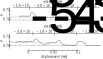
\includegraphics[scale=1]{../Figures_chap_intro/speed_mu.pdf}
\caption[Évolution de $\mu$ lors d'un saut de vitesse]{Évolution du coefficient de frottement dynamique en fonction de la vitesse (adapté de\,\cite{dieterich_modeling_1979}). Les échantillons étudiés sont des granodiorites d'une carrière californienne poncées avec du papier abrasif. La vitesse de déplacement varie au cours de l'expérience.}
\label{fig:speed_mu}
\end{figure}





Lorsqu'un solide est en glissement sur une surface, son coefficient de frottement évolue en fonction de la vitesse de glissement $V$ (Fig.\,\ref{fig:speed_mu}). En régime de glissement stable, $\mu$ est proportionnel au logarithme de  $V$\,\cite{ruina_slip_1983,stesky_mechanisms_1978,blanpied_frictional_1987,dieterich_direct_1994}. Lors d'un saut de vitesse positif, à temps court, $\mu$ augmente, puis relaxe à temps long vers une nouvelle valeur stable. Ce comportement provient de la concurrence de deux effets. L'augmentation initiale de $\mu$ est l'effet de la résistance intrinsèque des contacts\,\cite{dieterich_direct_1994}. La diminution qui s'en suit relève d'un mécanisme de fluage similaire à celui à l'œuvre dans le vieillissement d'une interface au repos.
L'interface est le siège d'une compétition entre le renouvellement des contacts par son glissement et le vieillissement des contacts sous une charge normale.
%Plus la vitesse est élevée, moins les contacts nouvellement formés ont le temps de vieillir avant d'être à nouveau brisés.


Ces deux dépendances logarithmiques de $\mu$ en temps et en vitesse peuvent être décrites par des loi empiriques telles que celle proposée par Dieterich et Ruina en 1979 et 1983, que nous présentons ci-dessous.

\subsubsection{Modèle de Dieterich et Ruina -- Rate-and-State}
\label{sec:rateandstate}


\begin{figure}[h!]
\centering
\includegraphics[scale=1]{../Figures_chap_intro/velocity_s_w.pdf}
\caption[Comportement du modèle Rate-and-State]{Schéma du comportement d'un système frictionnel suivant une loi Rate-and-State, en fonction des paramètres $A$ et $B$ du modèle (adapté de\,\cite{zhang_frictional_2022}). La courbe rouge (resp. bleue) présente une friction renforcée (resp. affaiblie) par la vitesse.}
\label{fig:velocity_s_w}
\end{figure}

\newpage

Le modèle de Dieterich et Ruina\,\cite{dieterich_modeling_1979,ruina_slip_1983} est un modèle \textit{Rate-and-State} (\textit{taux-état}, rarement traduit dans la littérature), reliant le coefficient de frottement $\mu$ à la vitesse de glissement $V$ et à une fonction d'état $\theta$, selon l'équation 

\begin{equation}
\mu = \mu_0+A\ln\left(1+\frac{V}{V_0}\right)+B\ln\left(1+\frac{\theta}{\theta_0}\right)
\end{equation}


La loi décrite ici étant empirique, son interprétation physique est sujette à des réserves\,\cite{dieterich_direct_1994}. Il est cependant possible d'en trouver des justifications microscopiques\,\cite{baumberger_physical_1999, nakatani_conceptual_2001,chen_microphysically_2017}. Ainsi $\theta$ est généralement interprété comme l'âge des microcontacts formés entre les deux solides. Les constantes $\theta_0$, $\mu_0$ et $V_0$ sont déterminées expérimentalement.

Cette équation doit être couplée avec une équation d'état modèle pour l'évolution de $\theta$. L'équation proposée par Dieterich considère que l'âge des contacts évolue selon l'équation

\begin{equation}
\diff{\theta}{t} = 1-\frac{\theta V}{D_c}
\end{equation}

La constante $D_c$, homogène à une longueur, correspond à la distance de glissement caractéristique nécessaire pour renouveler entièrement une population de contacts. Ce modèle permet d'exprimer à vitesse nulle le coefficient de frottement statique et de rendre compte de son augmentation logarithmique avec le temps.

\begin{equation}
\mu_s=\mu_0+B\ln(1+\theta/\theta_0)
\end{equation}

Lorsque le glissement se fait en régime stationnaire, $V$ est constante et $\theta = D_c/V$. Nous considérons les cas où $V/V_0\gg1$ et $D_c/V\theta_0\gg1$, hypothèses généralement valides pour les systèmes que nous étudions. Le cas général ainsi que les limites inverses de ces hypothèses sont traités dans la littérature\,\cite{bar-sinai_slow_2012, barsinai_velocitystrengthening_2014,bar-sinai_velocity-strengthening_2015}. Nous obtenons alors


\begin{equation}
\mu = \text{const.}+(A-B)\ln(V)
\end{equation}


Ce modèle met en évidence deux constantes $A$ et $B$, représentant respectivement la résistance au cisaillement des contacts et celle du vieillissement statique. L'effet de $A$, nommé \textit{effet direct}, est visible à temps court et va toujours dans le sens de la résistance au changement de vitesse. L'effet de $B$, ou \textit{effet indirect}, est visible à temps longs, lorsque le glissement est supérieur à $D_c$ (Fig.\,\ref{fig:velocity_s_w}). Lorsque le vieillissement est dominant, $B>A$, le frottement est d'autant plus faible que la vitesse est grande, il est dit affaibli par la vitesse (\textit{velocity weakening}). Dans le cas inverse, $A>B$, le frottement est renforcé par la vitesse (\textit{velocity strengthening}).

Ce modèle, bien que justifié par des considérations microscopiques, reste empirique. Aussi d'autres lois d'évolution de $\theta$ existent, représentant plus fidèlement le comportement de l'interface lorsqu'elle est soumise à des variations rapides de vitesse. Toutes cependant permettent de rendre compte d'un écart entre $\mu_s$ et $\mu_d$, et de l'apparition de deux régimes de déplacement, le glissement stable et le stick-slip\,\cite{ruina_slip_1983,nagata_revised_2012,aharonov_physicsbased_2018}.


\subsubsection{Instabilité de stick-slip}


\begin{figure}[htb]
\centering
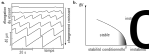
\includegraphics[scale=1]{../Figures_chap_intro/stability.pdf}
\caption[Diagramme de stabilité d'un mouvement de stick-slip]{\textbf{a.} Réponse d'un système masse-ressort posé sur un tapis roulant à vitesse constante. Lorsque la force normale décroît, le comportement de la masse effectue une transition entre un régime de stick-slip et un glissement permanent à vitesse variable, puis un glissement stable (adapté de\,\cite{baumberger_physical_1999}). \textbf{b.} Diagramme de stabilité schématique d'une interface affaiblie par la vitesse (adapté de \,\cite{scholz_earthquakes_1998}). Ce diagramme montre le saut de vitesse nécessaire afin de déstabiliser une interface en glissement stable, en fonction de la contrainte normale qui lui est appliquée. Le régime instable évolue en stick-slip quel que soit la perturbation de vitesse, tandis que le régime de stabilité conditionnelle n'évolue en stick-slip que si le saut de vitesse est suffisant.}
\label{fig:ss2}
\end{figure}


Dans le cas d'une interface à frottement renforcé par la vitesse, un mouvement de glissement est intrinsèquement stable. Une fluctuation de vitesse se traduit par un changement de vitesse de glissement stable. Une interface à frottement affaibli par la vitesse en revanche peut exhiber un comportement instable de stick-slip, comme conséquence de l'existence d'un coefficient de frottement dynamique inférieur au coefficient de frottement statique (Sec.\,\ref{sec:ss1}, Fig.\,\ref{fig:ss2}a). Ce comportement instable en vitesse est bien décrit par une bifurcation de Hopf\,\cite{rice_stability_1983,gu_slip_1984,heslot_creep_1994}. Si l'on considère un écart de vitesse $\Delta V$ appliqué à une interface en glissement stable, et $\sigma$ la pression normale appliquée sur l'aire de contact apparente $A$, il est possible de définir une valeur critique $\sigma_c$ de cette pression à laquelle le comportement du système passe d'un régime toujours instable à un régime conditionnellement stable (Fig\,\ref{fig:ss2}b).


Cette analyse de stabilité met en avant l'existence d'interfaces toujours en glissement stable car renforcées par la vitesse, et d'interfaces toujours instables car affaiblies par la vitesse et dans la zone instable du diagramme de bifurcation. Le modèle prédit également l'existence d'interfaces affaiblies par la vitesse, conditionnellement stables, nécessitant une fluctuation de vitesse pour entrer dans un régime de stick-slip. Cette fluctuation peut consister en la rupture partielle d'une interface, la portion instable de celle-ci entraînant une déstabilisation de sa portion conditionnellement stable. La détermination du caractère renforcé ou affaibli par la vitesse des portions de failles est à ce titre un enjeu majeur de l'étude des failles.




Le modèle Rate-and-State, couplé à une équation d'état, permet une bonne description de la dynamique d'une interface frictionnelle. Sa principale limitation réside dans son aspect empirique, nécessitant des ajustements pour déterminer les constantes $A$ et $B$ pour chaque système étudié. Dans un système de failles réelles, la connaissance des phénomènes à l'origine de leurs variations est nécessaire à l'étude et la prévision de la stabilité du mouvement. De plus les modèles présentés ne décrivent que le mouvement moyen de l'interface, celui du centre de masse du système, et ignorent son extension spatiale.

Cette dernière problématique soulève la question du mécanisme par lequel le mouvement s'initie. En effet cette initiation n'étant pas instantanée, elle doit s'accompagner d'un phénomène propagatif. Ce phénomène est la propagation d'une rupture interfaciale affaiblissant de proche en proche les microcontacts et permettant la mise en glissement de l'interface.


